Process aware information systems (PAIS) are becoming more and more widespread. These information systems log huge amounts of events and even more event data can be extracted from all other kinds of ubiquitous organizational databases. Even this complex task is becoming easier and better supported with current research. Additionally, due to the current Big Data craze, many other types of data sets are in need of analysis.

To conduct such analyses the L* lifecycle model for process mining \cite{van2011process} can be employed. It is composed of five steps. At first the project obviously needs to be planned and justified. Then, event data is extracted and analysis goals like improvement of certain KPIs (key performance indicators) are determined. As the third step, control-flow models are discovered, compared and reasoned about. Starting with this model a great variety of different approaches can be applied to gain insights about other perspectives like time, data-flow, resources and process context.
Finally, but this may only be possible for very structured processes (also called lasagna processes), operational support can be derived from the analyzed historical data and applied to active cases.

Two important activities in this lifecycle are conformance checking and performance analysis.
For conformance checking different techniques have been proposed. Footprint based conformance compares the possible behavior of log and model through a directly follows abstraction. This measure takes into account fitness as well as precision, so it is not very specific. With token replay based conformance checking, the number of produced, consumed, missing and remaining tokens is counted. This measures fitness but is influenced by the simplicity of the model because models with redundant places and the same behavior achieve a higher value. Lastly, alignment based conformance is the state of the art approach to obtain stable fitness values. Places and transitions are also visually ranked by their level of conformance. This general technique has also been improved over time with decomposition and re-composition concepts to mainly increase performance and scalability.

Performance analysis is usually alignment based. The sync moves in the alignment are mapped to the events in the log and time differences are used to calculate sojourn time on places and execution times for transitions if additional event lifecycle information is present. Often, only average times and frequencies along with the standard deviation are given.

However, real-life processes are rarely static and may exhibit many interesting patterns which are lost in averages when the perspectives are not fine grained enough.
\begin{figure}
    \centering
    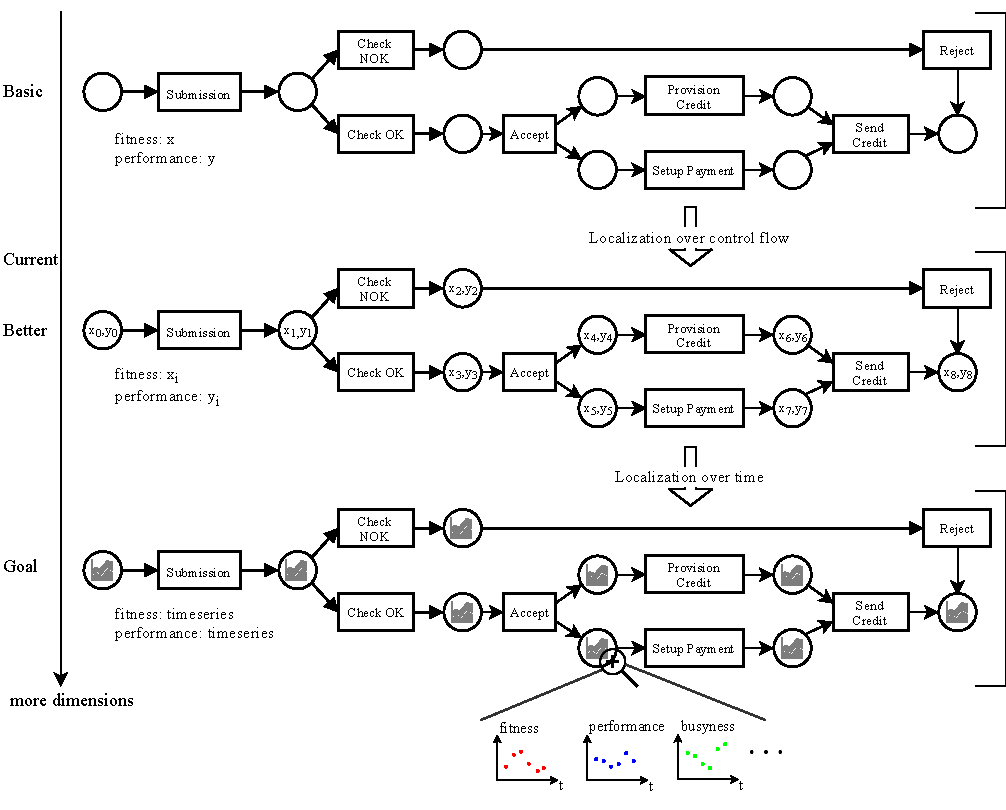
\includegraphics[width=\textwidth]{figures/introduction/bigschematic_v3.pdf}
    \caption{Schematic of the approach}
    \label{fig:bigschematic}
\end{figure}
As an example take the model given in Figure \ref{fig:bigschematic}. It describes a small credit application process where every application starts with a submission. Then, the credit history of the applicant is checked. If the result is negative, the application should be rejected, if not, accepted. After accepting, the credit is provisioned and the payment is setup in any order. Finally, the credit is sent. The information system logs the credit amount for cases, time and type of activity for events but no resource information. Now assume a certain employee is not following protocol. Whenever the load at his position is high and no one notices, he simply accepts low value applications where the credit history check was negative. Additionally, he actively delays high value applications making them wait for acceptance longer. All of this only happens for a short part of the whole logged time span.

To discover such a complex pattern in the event data given the model, a combination of many perspectives is necessary. More specifically,
\begin{itemize}
    \item conformance \textemdash \ acceptance of applications which should be rejected is a conformance problem
    \item performance \textemdash \ the delayed applications are a performance problem
    \item data \textemdash \ only low value applications deviate and only high value applications are delayed
    \item process context (busyness) \textemdash \ all of this only happens when the affected places are busy, i.e. many cases are currently waiting there
\end{itemize}
Furthermore, these perspectives need to be measured fine grained enough. Without adding a dimension, there would only be one number per perspective for the whole log and model. For example, the average fitness, the average case duration, the case attributes and the number of cases. By localizing the perspectives to places (along the control-flow dimension), these metrics can be calculated for each place. This is an improvement but not enough to find this pattern because, due to this phenomenon only occurring for a short while, it may still be drowned out in averages over the whole time span. When further localizing along the time dimension, the analysis will finally be fine enough to single out this pattern when correlating the metrics which are now timeseries for each place.

That is why we present an approach to approximate conformance, performance and process context locally in the model and discretized over time. Section two will cover the preliminaries necessary for the concept which will be presented in section three. Following that, the implementation in ProM will be shown. Then, the approach will evaluated on a real-life dataset in section five. Second to last, related work will be discussed and the report is concluded with a conclusion.